\chapter{F-TRACT}\label{ch:ftract}

The entry point of this thesis is the paper \textit{Communication dynamics in the human connectome shape the cortex-wide propagation of direct electrical stimulation} by Sequin et al., published in 2022. It shows that the network communication models discussed in Chapter \ref{ch:networks} computed using structural connectome based on DW-MRI can, up to some degree, explain the propagation of focal electrical stimulation through the brain. 

The main question of this thesis is whether it is possible to apply the methodology used by Seguin et al. to find correlations between the response to an intracranial stimulation and network communication models to TMS-EEG data. Before diving into that, let us devote this chapter to a closer investigation of the aforementioned paper and our experiments with the Functional Brain Tractography project (F-TRACT) iEEG functional data.  

\section{F-TRACT iEEG functional data}

The Functional Brain Tractography project (F-TRACT)\footnote{\url{https://f-tract.eu/}} summary dataset used in this section was prepared by Jedynak et el. \cite{jedynak_f-tract_2023} and it is available from the EBRAINS platform.\footnote{\url{https://doi.org/10.25493/H0JJ-0YD}} It consists of several matrices characterizing the brain's response to intracranial electrical stimulation.

The F-TRACT project aggregated iEEG data from 550 patients with drug-resistant epilepsy measured during $29\,055$ stimulations using 2.77 million pairs of intracerebral depth electrodes. In order to mitigate the impact of epileptogenic processes in further analyses, recordings with a high likelihood of pathological activity were excluded. The results were projected onto a number of parcellations. We use Glasser parcellation in this chapter (more in Section \ref{sec:parcellations}). \cite{jedynak_f-tract_2023,seguin_communication_2023} 

The recorded evoked potentials were baseline corrected\footnote{Baseline correction is based on utilizing EEG activity from a baseline period—before an external event—to adjust activity during a post-stimulus interval.} and $z$-scored. Stimulus response was considered significant if the $z$-scored evoked potential over $z = 5$ was observed. The response amplitude was defined as the first peak of $z$-scored evoked potential above the $z = 5$ threshold. Using that, two whole-brain group-level matrices were constructed. Entries $P_{ij} \in [0,1]$ of response probability matrix $P$ characterize the probability that we observe a significant response as described above in ROI $j$ after stimulation of $i$. Entries $A_{ij} \in \mathbb{R}_{>0}$ of response amplitude matrix $A$ capture the median response amplitude of significant responses.

It is important to mention that the dataset available on EBRAINS publishes the response probability and amplitude matrices in two versions, one considering responses up to 50 ms after the stimulus and the other up to 200 ms after the stimulus. However, Sequin et al. used the responses up to 800 ms after the stimulation.\footnote{They used the 200 ms version in robustness analysis, it can be found in the Supplementary information of the paper. \cite{seguin_communication_2023} } That might be a source of discrepancy in the results.

\section{Results}\label{sec:ftract_results}

In this section, we present the results of our replication of the work by Sequin et al. \cite{seguin_communication_2023}. There is a key difference between our results and the original paper in that we used not only structural connectivity weights derived from streamline counts between individual ROI, but also streamline lengths. We show that the lengths correlate very well with the response probability.

We used several structural connectivity matrices obtained from several datasets. More about the construction of these specific matrices and experiments with them can be found in Chapter \ref{ch:SC_indepth}. All the matrices were pruned to keep graph density $25\%$.

For each dataset, we calculated the communication metrics matrices described in Chapter \ref{ch:networks}. Table \ref{tab:matrices_usage} shows which matrices were used as inputs for the metrics. It is an important comparison because we want to know if the communication metrics bring any advantage over plain structural connectivity or Euclidean distances, i.e. do we get anything new by using communication metrics with these inputs over the inputs themselves? 

\begin{table}
    \centering
    \begin{tabular}{l| l}
        metric & matrices  \\
        \hline
        $SPE$   & $SC_L$ \\
        $SPE_W$ & $1/SC_W$ instead of $SC_L$ \\
        $COM$   & $SC_W$ \\
        $SI$    & $SC_W$ for navigation, $ED$ for path length \\
        $SI_L$  & $SC_W$ for navigation, $SC_L$ for path length \\
        $NAV$   & $SC_W$ only to get connectedness, $ED$ ($SC_L$ for path length) \\ 
        $DIF$   & $SC_W$ \\
    \end{tabular}
    \caption[Matrices used in communication metrics calculation]{Matrices used in communication metrics calculation, $SC_W$ structural connectivity weights, $SC_L$ structural connectivity lengths, $ED$ Euclidean distances. For navigation efficiency ($NAV$) we used $SC_L$ for path length calculation if available, otherwise $ED$.}
    \label{tab:matrices_usage}
\end{table}

We used the Spearman correlation coefficient of the response matrix and structural and communication matrices to evaluate the relationship between structure and function. It is a reasonable choice because we want to see if the response probability is higher in regions that are \uv{easier to access}, but we do not expect the relationship to be linear, thus we do not use the Pearson correlation coefficient. Seguin et al. used Spearman correlation as well, so the results are comparable.

We always calculated full and partial correlation, the latter with the influence of Euclidean distance controlled. The idea behind the partial correlation calculation is that we want to investigate how much of the response variance could be explained that was not accounted for by spatial proximity.

All the correlations were calculated for all ROI pairs (i. e. the whole matrix) where the response probability/amplitude was not nan (enough stimulations, enough significant responses, not too close, if close pairs excluded).

\subsection{Robustenss in structural connectome selection}\label{sec:sc-robustness_ftract}

First of all, the correlations are robust to structural connectome selection. Figure \ref{fig:ftract_alldata_long_probabilities} shows the correlations of response probabilities with structural matrices and communication metrics. Figure \ref{fig:ftract_alldata_long_amplitudes} shows the same for response amplitudes. We can see that there are differences in results based on the dataset and group-averaging method selection, but there are significant correlations for all of them and differences are generally rather small for most of the communication metrics.\footnote{Change of response length (50 ms, 200 ms) or excluding close pairs or regions do not reveal any new information.} Because of that, we present the rest of the results with only the Mica-Mics dataset and Rosen and Halgren's group averaging method for simplicity. \TODO[kde se dá kouknout na další výsledky]

We chose the Mica-Mics dataset because it provides Schaefer200 parcellation as well, so we can use the same dataset here and in the experiments with TMS-EEG data (Chapter \ref{ch:pytepfit}). The Rosen and Halgren's group averaging method is selected because it seems that it sometimes (e. g. $SC_W$ and $SPE_W$ in Figure \ref{fig:ftract_alldata_long_amplitudes}) results in higher correlations than the other approaches.

\begin{figure}
    \centering
    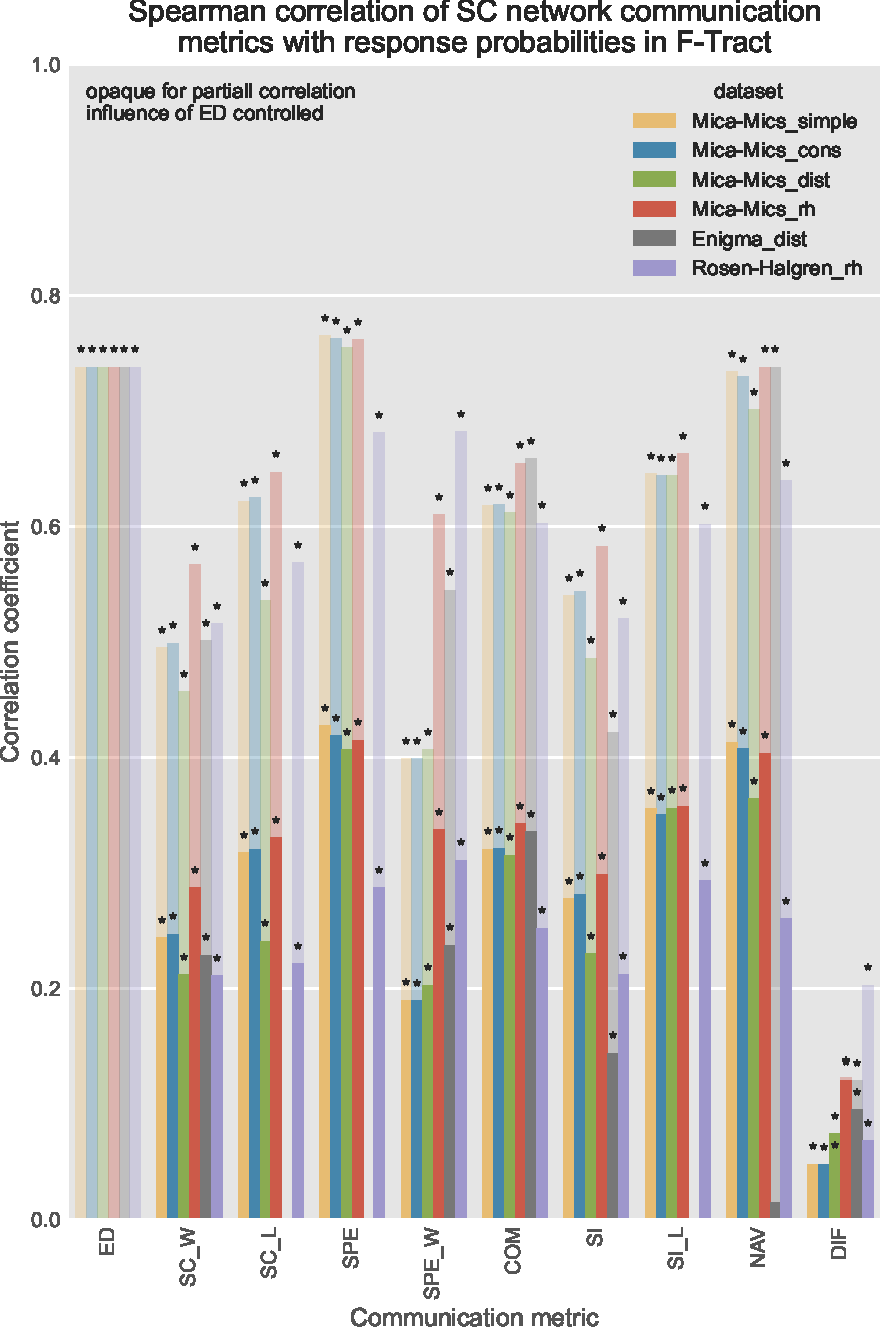
\includegraphics[width=0.93\textwidth]{images/nootebook_generated/ftract_results/MNI-HCP-MMP1/5/ED0/0.25/long/Spearman_correlation_of_SC_network_communication_metrics_with_response_probabilities_in_F-Tract.pdf}
    \caption[F-TRACT probability correlations - all $SC$ matrices]{Correlations (absolute value) of response probability (200~ms response) and structural connectivity and derived communication metrics. Asterisks denote a significant correlation ($p<0.05$).}
    \label{fig:ftract_alldata_long_probabilities}
\end{figure}


\begin{figure}
    \centering
    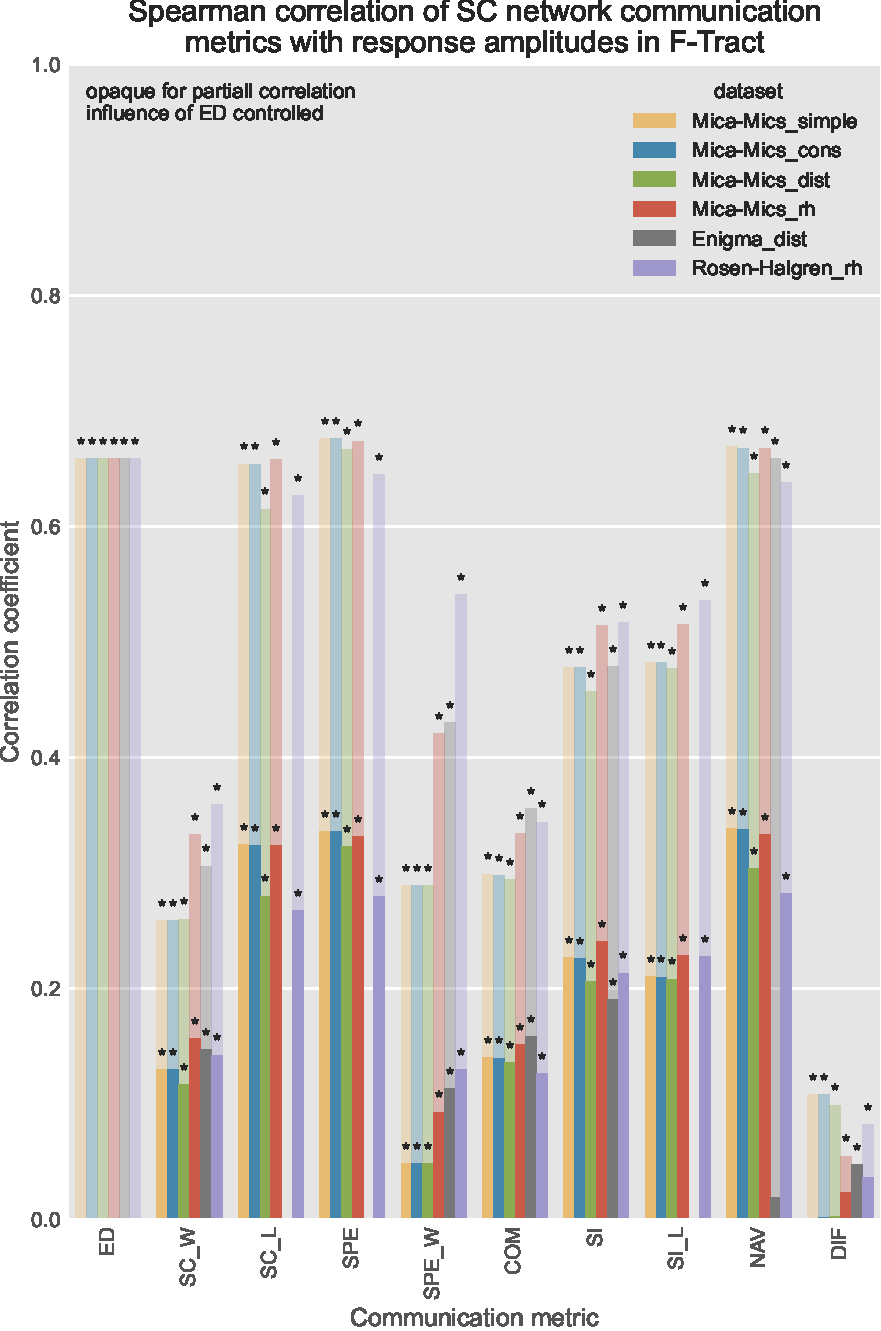
\includegraphics[width=0.93\textwidth]{images/nootebook_generated/ftract_results/MNI-HCP-MMP1/5/ED0/0.25/long/Spearman_correlation_of_SC_network_communication_metrics_with_response_amplitudes_in_F-Tract.pdf}
    \caption[F-TRACT amplitude correlations - all $SC$ matrices]{Correlations (absolute value) of response amplitude (200~ms response) and structural connectivity and derived communication metrics. Asterisks denote a significant correlation ($p<0.05$).}
    \label{fig:ftract_alldata_long_amplitudes}
\end{figure}


\subsection{Response vs communication metrics}

Could communication metrics be used to explain the response probability and amplitude of reaction on stimulus in individual ROIs? That was the main question of Seguin et al. \cite{seguin_communication_2023} and it is the focus of this thesis. We overall confirmed the results of Seguin et al. that there are correlations between the communication metrics and response probability and amplitude, and that those can overcome the correlations with the plain weights of the structural connectome. 

However, Seguin et al. did not use structural connectivity lengths, which appear to be correlated with both response probability (see Figure \ref{fig:ftract_alldata_long_probabilities}, column $SC_L$) and response amplitude (see Figure \ref{fig:ftract_alldata_long_amplitudes}, column $SC_L$) even better than the structural connectivity weights. It is a contribution of our work that we included structural connectivity lengths in the analysis. 

Let us look closer at the correlations for response probability and amplitude in the following subsections.

\subsubsection{Response probability}\label{sec:probability_F-Tract}

Seguin et al. showed a correlation of response probability with Euclidean distance of approximately $0.6$. Figure \ref{fig:ftract_alldata_long_probabilities} shows that we found an even higher correlation. This might be caused by the fact that Seguin et al. excluded pairs of ROIs that are closer than 20 mm from the analysis. They also considered the responses up to 800 ms after the stimulation. The Supplementary material of their paper shows the results without the close pairs exclusion and with 200 ms responses; both are closer to ours. Therefore we think that these factors may be a cause of overall higher correlations in our results. We also tried to exclude the close pairs (\TODO[kde to najít]), the correlations were generally slightly lower in that case. 

It can be seen in Figure \ref{fig:ftract_alldata_long_probabilities} that there are correlations between the response probability and structural connectivity and communication metrics. However, it is not possible to order all the metrics from the best to the worst one because of the differences in the input matrices (they differ in dataset and group-averaging method). Despite that, let us describe the main findings.

The shortest path efficiency $SPE$ calculated using the structural connectivity lengths yields the highest correlations with response probability across all parameter settings we tried. The correlation is consistently $>0.6$ (often $>0.7$) for both 50 ms and 200 ms responses, various datasets and it stays high if we exclude close pairs or ROIs from the analysis.

Another metric with a consistently high correlation with response probability is the navigation efficiency $NAV$ based on the idea of signal navigation in each node to the neighbor with the shortest Euclidean distance to the target. The length of the final path was calculated using structural connectivity lengths, which might be the reason for its similarity to the shortest path efficiency.

The third metric we want to discuss is communicability $COM$. It does not result in absolute correlations as high as the shortest path efficiency $SPE$ and the navigation efficiency $NAV$, but it is better than the structural connectivity weights that are the only input of this metric. 

Our results also agree with Seguin et al. that the diffusion efficiency $DIF$ is not useful for the characterization of the response probability because of low and often non-significant correlations. 

\subsubsection{Response amplitude}

First of all, the response amplitude matrix is sparser than the response probability matrix because amplitudes were included in the analysis only for regions with at least 100 significant responses. That may be a source of uncertainty in the response amplitude analysis. 

An interesting observation is that the structural connectivity lengths correlate with the amplitude much better than the structural connectivity weights and the difference is higher than for the response probability discussed in the previous section.

Generally, the response amplitudes correlate less with all the communication matrices. We do not discuss amplitudes closer in this section because, as shown in Chapter \ref{ch:pytepfit}, they are not useful in the generalization of the approach to TMS-EEG.

\subsection{Short (50 ms) vs long (200 ms) responses}\label{sec:response-length_F-Tract}

The investigation of the influence of the response length is important for the application of this approach to the TMS-EEG data. The TMS coil makes a sound when turned on, so the later responses in TMS-EEG data include the reaction of the brain to the auditory stimulus. 

Comparing Figure \ref{fig:ftract_mica_short_probabilities} and Figure \ref{fig:ftract_mica_long_probabilities} the structural connectivity and communication matrices show very similar full correlation for both 50 and 200 ms responses. We can see that the shorter responses correlate more with Euclidean distance and the partial correlations with Euclidean distance control are lower. According to the results, it seems that the earlier responses are driven more by Euclidean distance, while the later responses exhibit more complex behavior. 

\begin{figure}
    \centering
    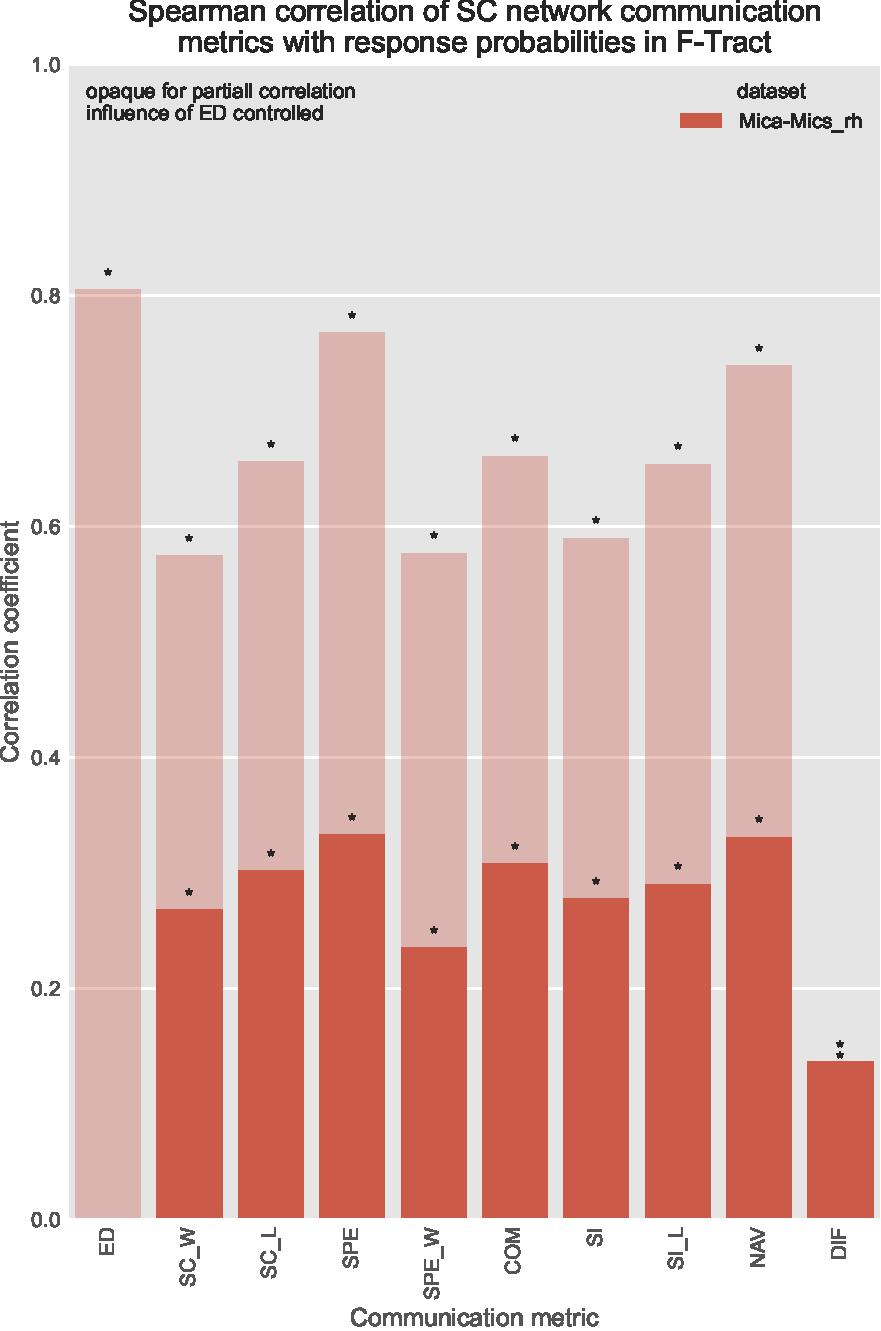
\includegraphics[width=0.93\textwidth]{images/nootebook_generated/ftract_results/MNI-HCP-MMP1/5/ED0/0.25/short/mica_rhSpearman_correlation_of_SC_network_communication_metrics_with_response_probabilities_in_F-Tract.pdf}
    \caption[F-TRACT probability correlations - Mica-Mics\_rh 50 ms]{Correlations (absolute value) of response probability (50~ms response) and structural connectivity and derived communication metrics. Asterisks denote a significant correlation ($p<0.05$).}
    \label{fig:ftract_mica_short_probabilities}
\end{figure}

\begin{figure}
    \centering
    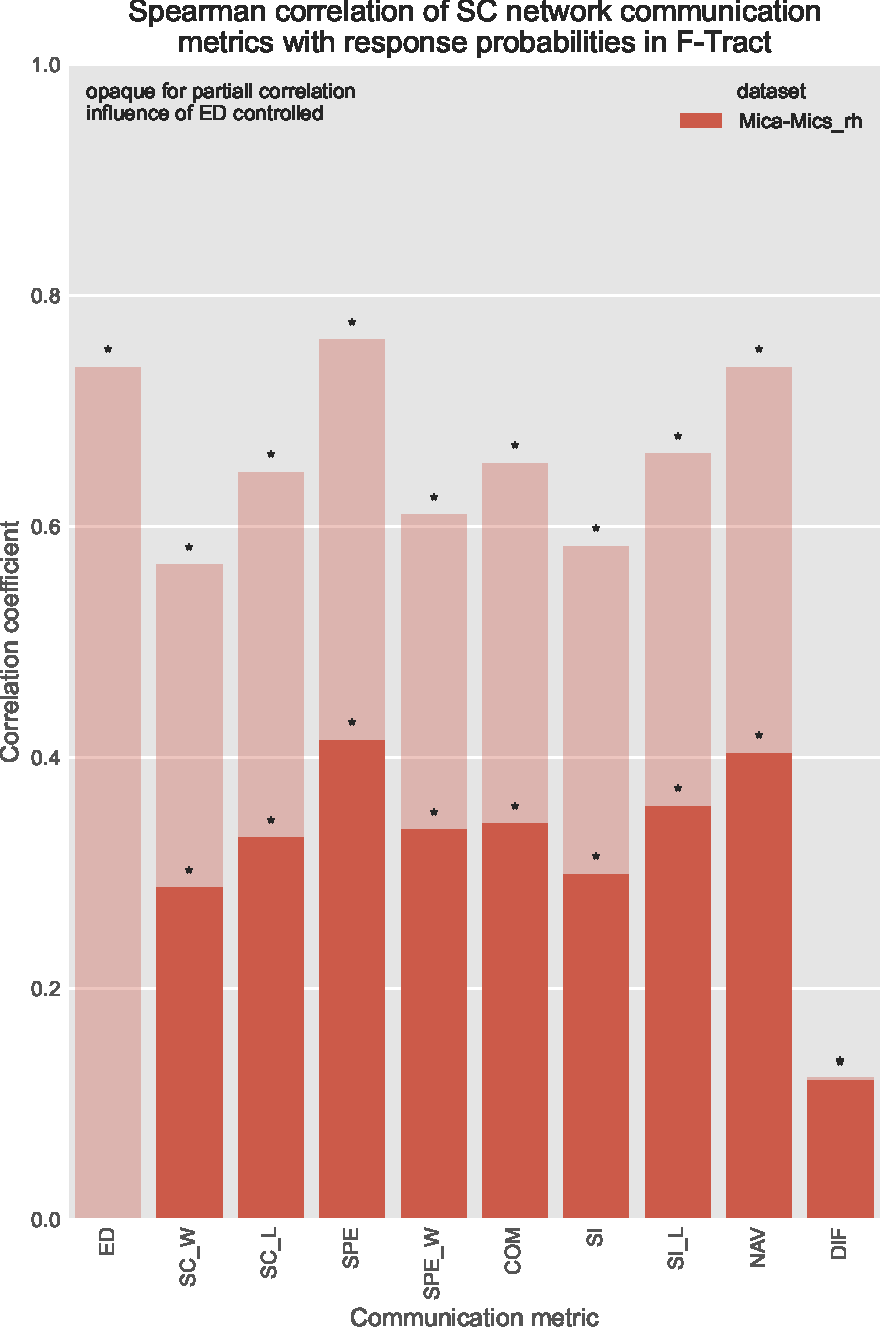
\includegraphics[width=0.93\textwidth]{images/nootebook_generated/ftract_results/MNI-HCP-MMP1/5/ED0/0.25/long/mica_rhSpearman_correlation_of_SC_network_communication_metrics_with_response_probabilities_in_F-Tract.pdf}
    \caption[F-TRACT probability correlations - Mica-Mics\_rh 200 ms]{Correlations (absolute value) of response probability (200~ms response) and structural connectivity and derived communication metrics. Asterisks denote a significant correlation ($p<0.05$).}
    \label{fig:ftract_mica_long_probabilities}
\end{figure}

\subsection{Response onset and peak delay}

Section \ref{sec:reponse_definition} discusses several options of \uv{response significance/strength} definition for TMS-EEG data. We confirmed Sequin et al.'s results showing a correlation between response probability and amplitude and the structural connectivity and communication metrics derived from it. However, the F-TRACT dataset also provides other characteristics of the responses, including response onset delay and response peak delay. Could those be used for response characterization and predicted using structural connectivity? We ran the analysis for them as well.

The partial correlations controlling for Euclidean distance are generally lower than $0.1$ and often not significant. For the 50 ms responses, the full correlations are generally lower than $0.2$, which we interpret as no relationship between the peak onset/delay and communication metrics in this case. However, the full correlations for 200 ms responses are significant and higher than $0.2$ for all communication metrics except the diffusion efficiency. For Euclidean distance, the correlation is $>0.4$ for both peak onset and delay. That suggests that there might be some relationship for longer responses and supports our idea of response characterization by its peaks in Section \ref{sec:reponse_definition}.

\subsection{Connected and unconnected regions}

The paper by Seguin et al. \cite{seguin_communication_2023} analyses the results not only for all region pairs, but also for connected and unconnected regions separately. We do not include this analysis because our main goal is an application of the approach to TMS-EEG datasets, for which it is not reasonable because we consider stimulation of a single site (not many different sites across the brain as here), so we have much less data.

\section{Results for primary motor cortex (M1) ROI}\label{sec:ftract_results_per_roi}

All the results presented above calculated the correlations for all ROI pairs together, expecting the stimulation of various ROIs. However, the TMS-EEG data we use in this thesis were measured during the stimulation of a single ROI, namely the left hemisphere's primary motor cortex (denoted M1), as stated in the data-describing paper from Biabani et al. \cite{biabani_characterizing_2019} Primary motor cortex in the left hemisphere is denoted L\_4 in Glasser parcellation. On the grounds of that, we selected only the row corresponding to L\_4 stimulation from the response probability matrix and the corresponding rows from the structural and communication matrices, and we calculated the correlations between these rows. 

Figure \ref{fig:ftract_mica_long_probabilities_L4} shows the results for the stimulation of M1 in the left hemisphere and 200 ms response. The results for the 50 ms response are very similar. Both show most of the full correlations above $0.6$ and partial correlations above $0.2$, with the shortest path efficiency $SPE$ having the highest full correlation with the response probability. Considering the partial correlations, the highest correlation is achieved with structural connectivity lengths $SC_L$.

\begin{figure}
    \centering
    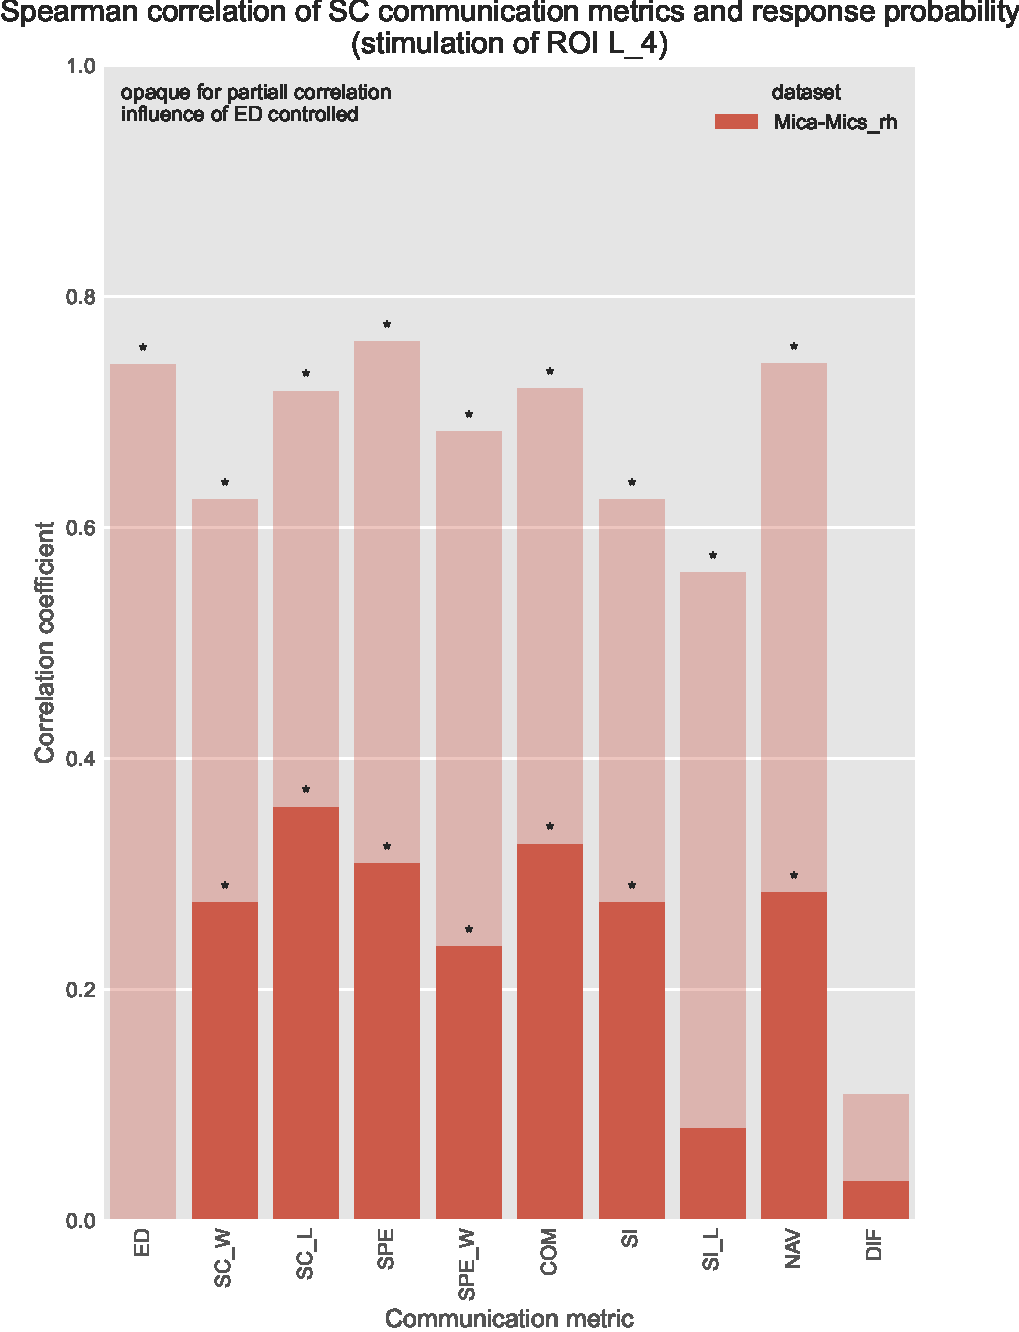
\includegraphics[width=\textwidth]{images/nootebook_generated/ftract_results_per_roi/long/MNI-HCP-MMP1/ED0/0.25/Spearman_correlation_of_SC_communication_metrics_and_response_probability_(stimulation_of_ROI_L_4).pdf}
    \caption[F-TRACT probability correlations - Mica-Mics\_rh L\_4]{Correlations (absolute value) of response probability (200~ms response) and structural connectivity and derived communication metrics. Asterisks denote a significant correlation ($p<0.05$).}
    \label{fig:ftract_mica_long_probabilities_L4}
\end{figure}

\subsection{Was the stimulation target really M1?}

Even though Biabani et al. \cite{biabani_characterizing_2019} declare they stimulated the primary motor cortex, the source-reconstruction of the TMS-EEG data by Momi et al. \cite{momi_tms-evoked_2023} suggest the stimulation of slightly different site, specifically L\_3b. This is further explained in Section \ref{sec:parcellations-mapping-stimulated_roi}. Here we just present the results for L\_3b stimulation in Figure \ref{fig:ftract_mica_long_probabilities_L3b}, so we can later use them for comparison.

\begin{figure}
    \centering
    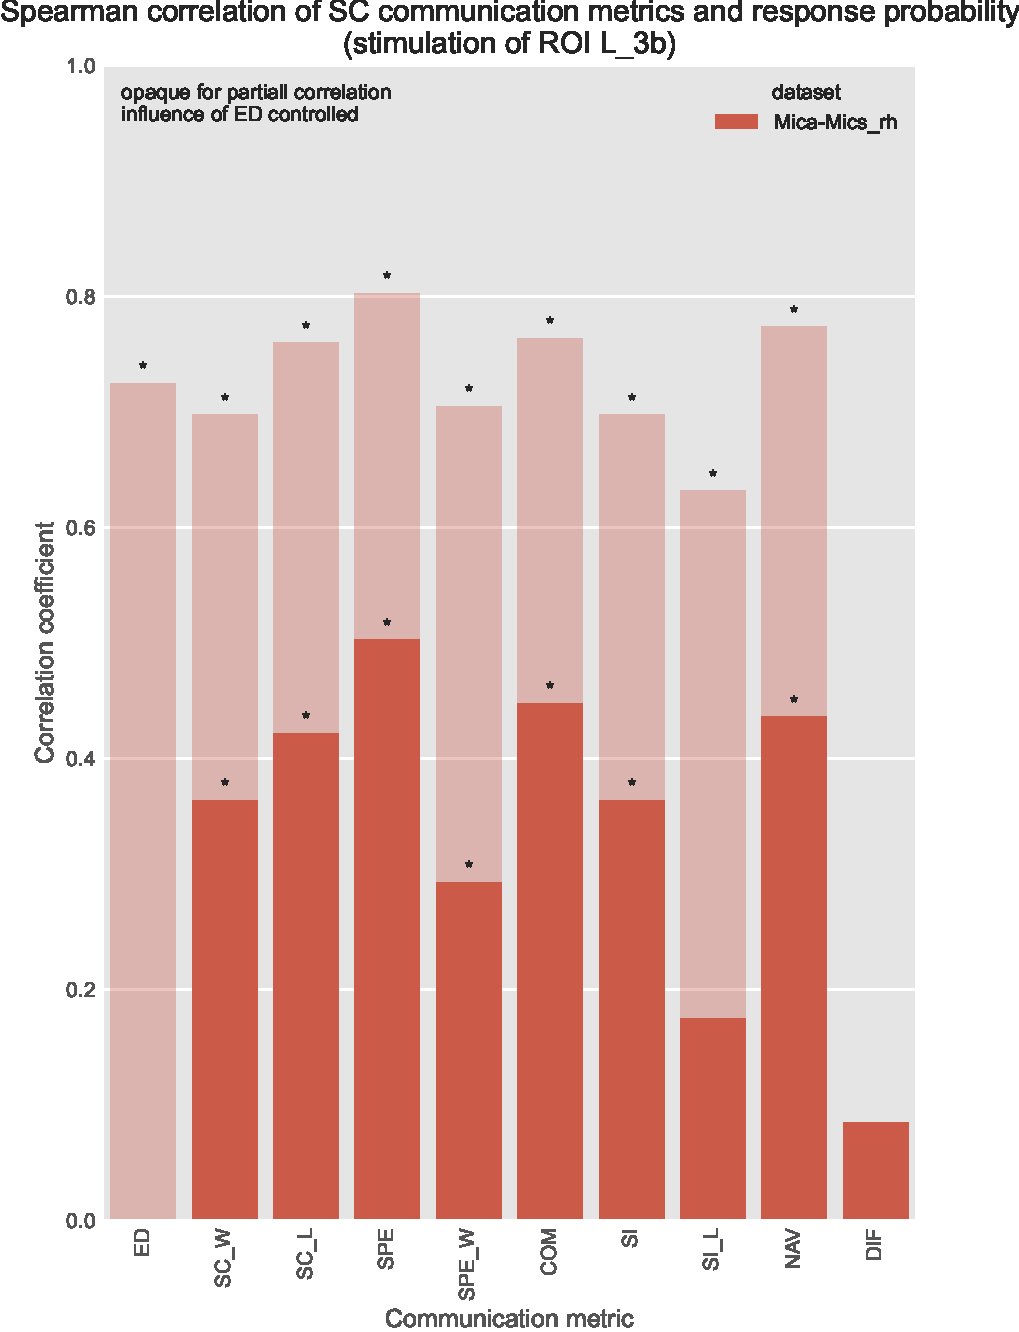
\includegraphics[width=\textwidth]{images/nootebook_generated/ftract_results_per_roi/long/MNI-HCP-MMP1/ED0/0.25/Spearman_correlation_of_SC_communication_metrics_and_response_probability_(stimulation_of_ROI_L_3b).pdf}
    \caption[F-TRACT probability correlations - Mica-Mics\_rh L\_3b]{Correlations (absolute value) of response probability (200~ms response) and structural connectivity and derived communication metrics. Asterisks denote a significant correlation ($p<0.05$).}
    \label{fig:ftract_mica_long_probabilities_L3b}
\end{figure}

The full correlations are overall even higher in this case than for the primary motor cortex stimulation (Figure \ref{fig:ftract_mica_long_probabilities_L4}) or the aggregated results (\ref{fig:ftract_mica_long_probabilities}). Regarding the communication metrics, the highest correlation is achieved with the shortest path efficiency (for both full and partial correlation), followed by communicability and navigation efficiency. Consistently with the previous results, the shortest path efficiency correlation with the probability response is higher than the correlation of the response with structural connectivity matrices.

The results for L\_4 and L\_3b confirm that it is reasonable to study correlations of stimulation responses with structural connectivity and communication metrics even if the stimulation was performed only at one site. That is an important finding, because TMS stimulation is often performed only at one site, and it is not possible to apply it to some ROIs (TMS can directly stimulate only 3 cm maximum depth from the surface of the head \cite{luber_using_2022}).